\begin{tutorial}{Швея Севера}

Начиная с $n=3$, все клетки на границе прямоугольника с панно будут черные, кроме одной, соседней с углом.  Такие клетки помечены крестиком на рисунке, где приведен пример для $n=15$. Если отбросить клетки на границе, получим прямоугольник, на границе которого все клетки белые, кроме одной, на рисунке такие клетки помечены кружком. Внутри снова черный прямоугольник, не считая одной белой клетки, и так далее. 

Поэтому панно отличается от картинки с концентрическими чередующимися черными и белыми прямоугольниками лишь по диагонали $D$ из крестиков и кружков. Эта диагональ проходит от  первой снаружи клетки, помеченной крестиком, к центру картинки.

\noindent\medskip\centerline{
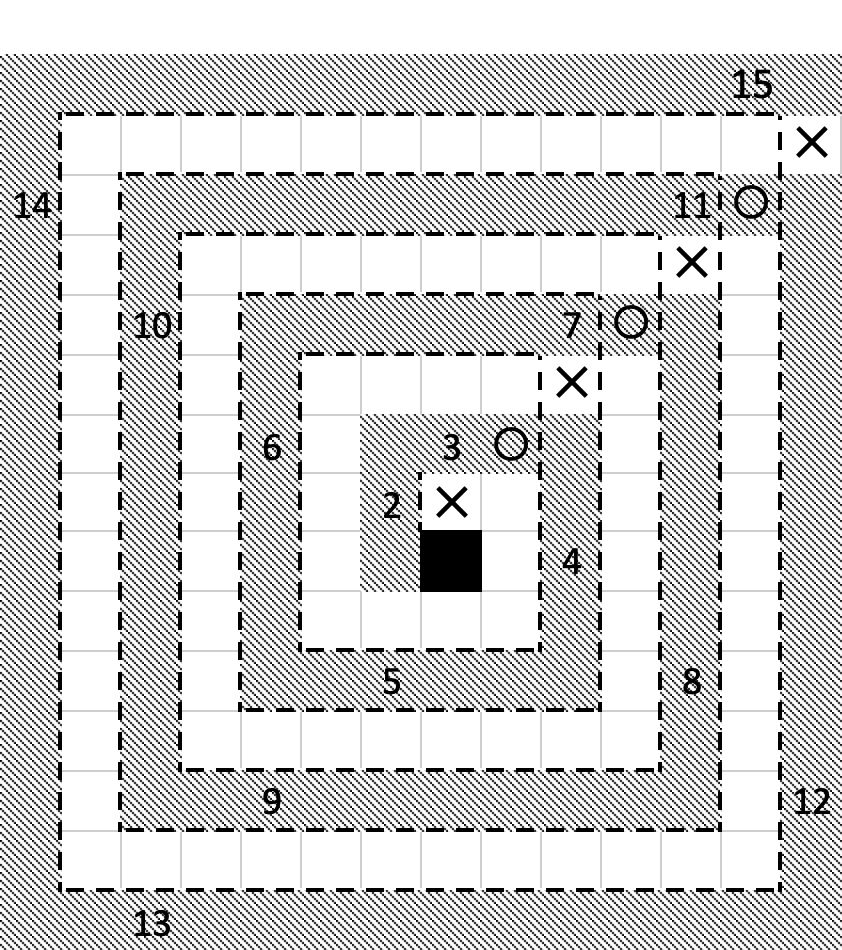
\includegraphics[bb=0 0 7.2in 7in, scale=.3]{loskut_tut_1.png}
\qquad
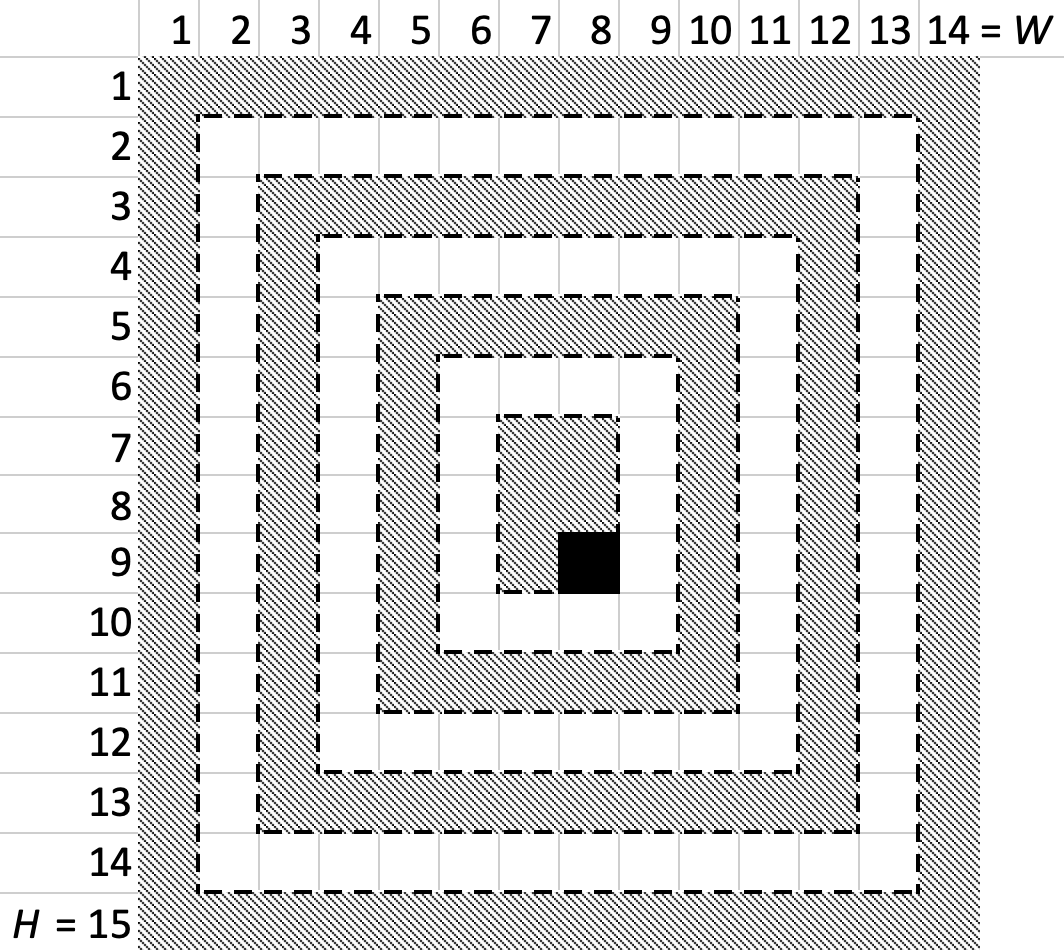
\includegraphics[bb=0 0 7.2in 7in, scale=.3]{loskut_tut_2.png}
}\\
Будем считать, что значение 1 (черный цвет) соответствует истине, а 0 (белый цвет) --- лжи. Так как на диагонали цвет клетки обратен тому, что получается для концентрических прямоугольников, то на панно цвет клетки $A(x,y)$ совпадает с истинностью утверждения:
<<(расстояние от клетки $A$ до ближайшей границы четное) \texttt{XOR}~(клетка $A$ лежит на диагонали $D$)>>, где \texttt{XOR}~--- операция <<исключающее ИЛИ>>.


\end{tutorial}
